\documentclass{edm_template}
%\documentclass{llncs}
\usepackage{graphicx, booktabs}
\usepackage[hang]{subfigure}
\usepackage{amsmath}

%\bibliographystyle{plain}
\bibliographystyle{abbrv}
\pagestyle{plain}

\title{Adaptive Practice of Facts in Domains with Varied Prior Knowledge}

\numberofauthors{3}

\author{
\alignauthor Jan Papou\v{s}ek\\
       \affaddr{Masaryk University Brno}\\
       \email{jan.papousek@mail.muni.cz}
\alignauthor Radek Pel\'{a}nek\\
       \affaddr{Masaryk University Brno}\\
       \email{pelanek@fi.muni.cz}
\alignauthor V\'{i}t Stanislav\\
       \affaddr{Masaryk University Brno}\\
       \email{slaweet@mail.muni.cz}
}

\begin{document}

\maketitle

\begin{abstract}
  We propose a modular approach to development of a computerized adaptive
  practice system for learning of facts in areas with widely varying prior
  knowledge: decomposing the system into estimation of prior knowledge,
  estimation of current knowledge, and selection of questions. We describe
  specific realization of the system for geography learning and use data from
  the developed system for evaluation of different student models for knowledge
  estimation. We argue that variants of the Elo rating systems and Performance
  factor analysis are suitable for this kind of educational system, as they
  provide good accuracy and at the same time are easy to apply in an online
  system.
\end{abstract}

%{{{ introduction

\section{Introduction}

Computerized adaptive practice~\cite{klinkenberg2011computer} aims at providing
students with practice in an adaptive way according to their skill, i.e. to
provide the students with tasks that are most useful to them. Our aim is to
make the development of such a system as automated as possible, particularly to
enable the system to learn the relevant aspects of the domain from the data so
that there is no need to rely on domain experts. This aspect is especially
important for development of systems for small target groups of students, e.g.
systems dealing with specialised topics or languages spoken by relatively small
number of people (like Czech).

This work is focuses on the development of adaptive systems for learning of
facts. In the terminology of the ``knowledge learning instruction
framework''~\cite{koedinger2012knowledge} we focus on constant-constant
knowledge components, i.e. knowledge components with a constant application
condition and a constant response. We are particularly concerned with learning of facts in
areas where students are expected to have nontrivial and highly varying prior
knowledge, e.g. geography, biology (fauna, flora), human anatomy, or foreign
language vocabulary. To show the usefulness of focusing on estimation of
prior knowledge, Figure~\ref{fig:africa} visualizes the significant differences
in prior knowledge of African countries.

\begin{figure}[t]
  \centering

  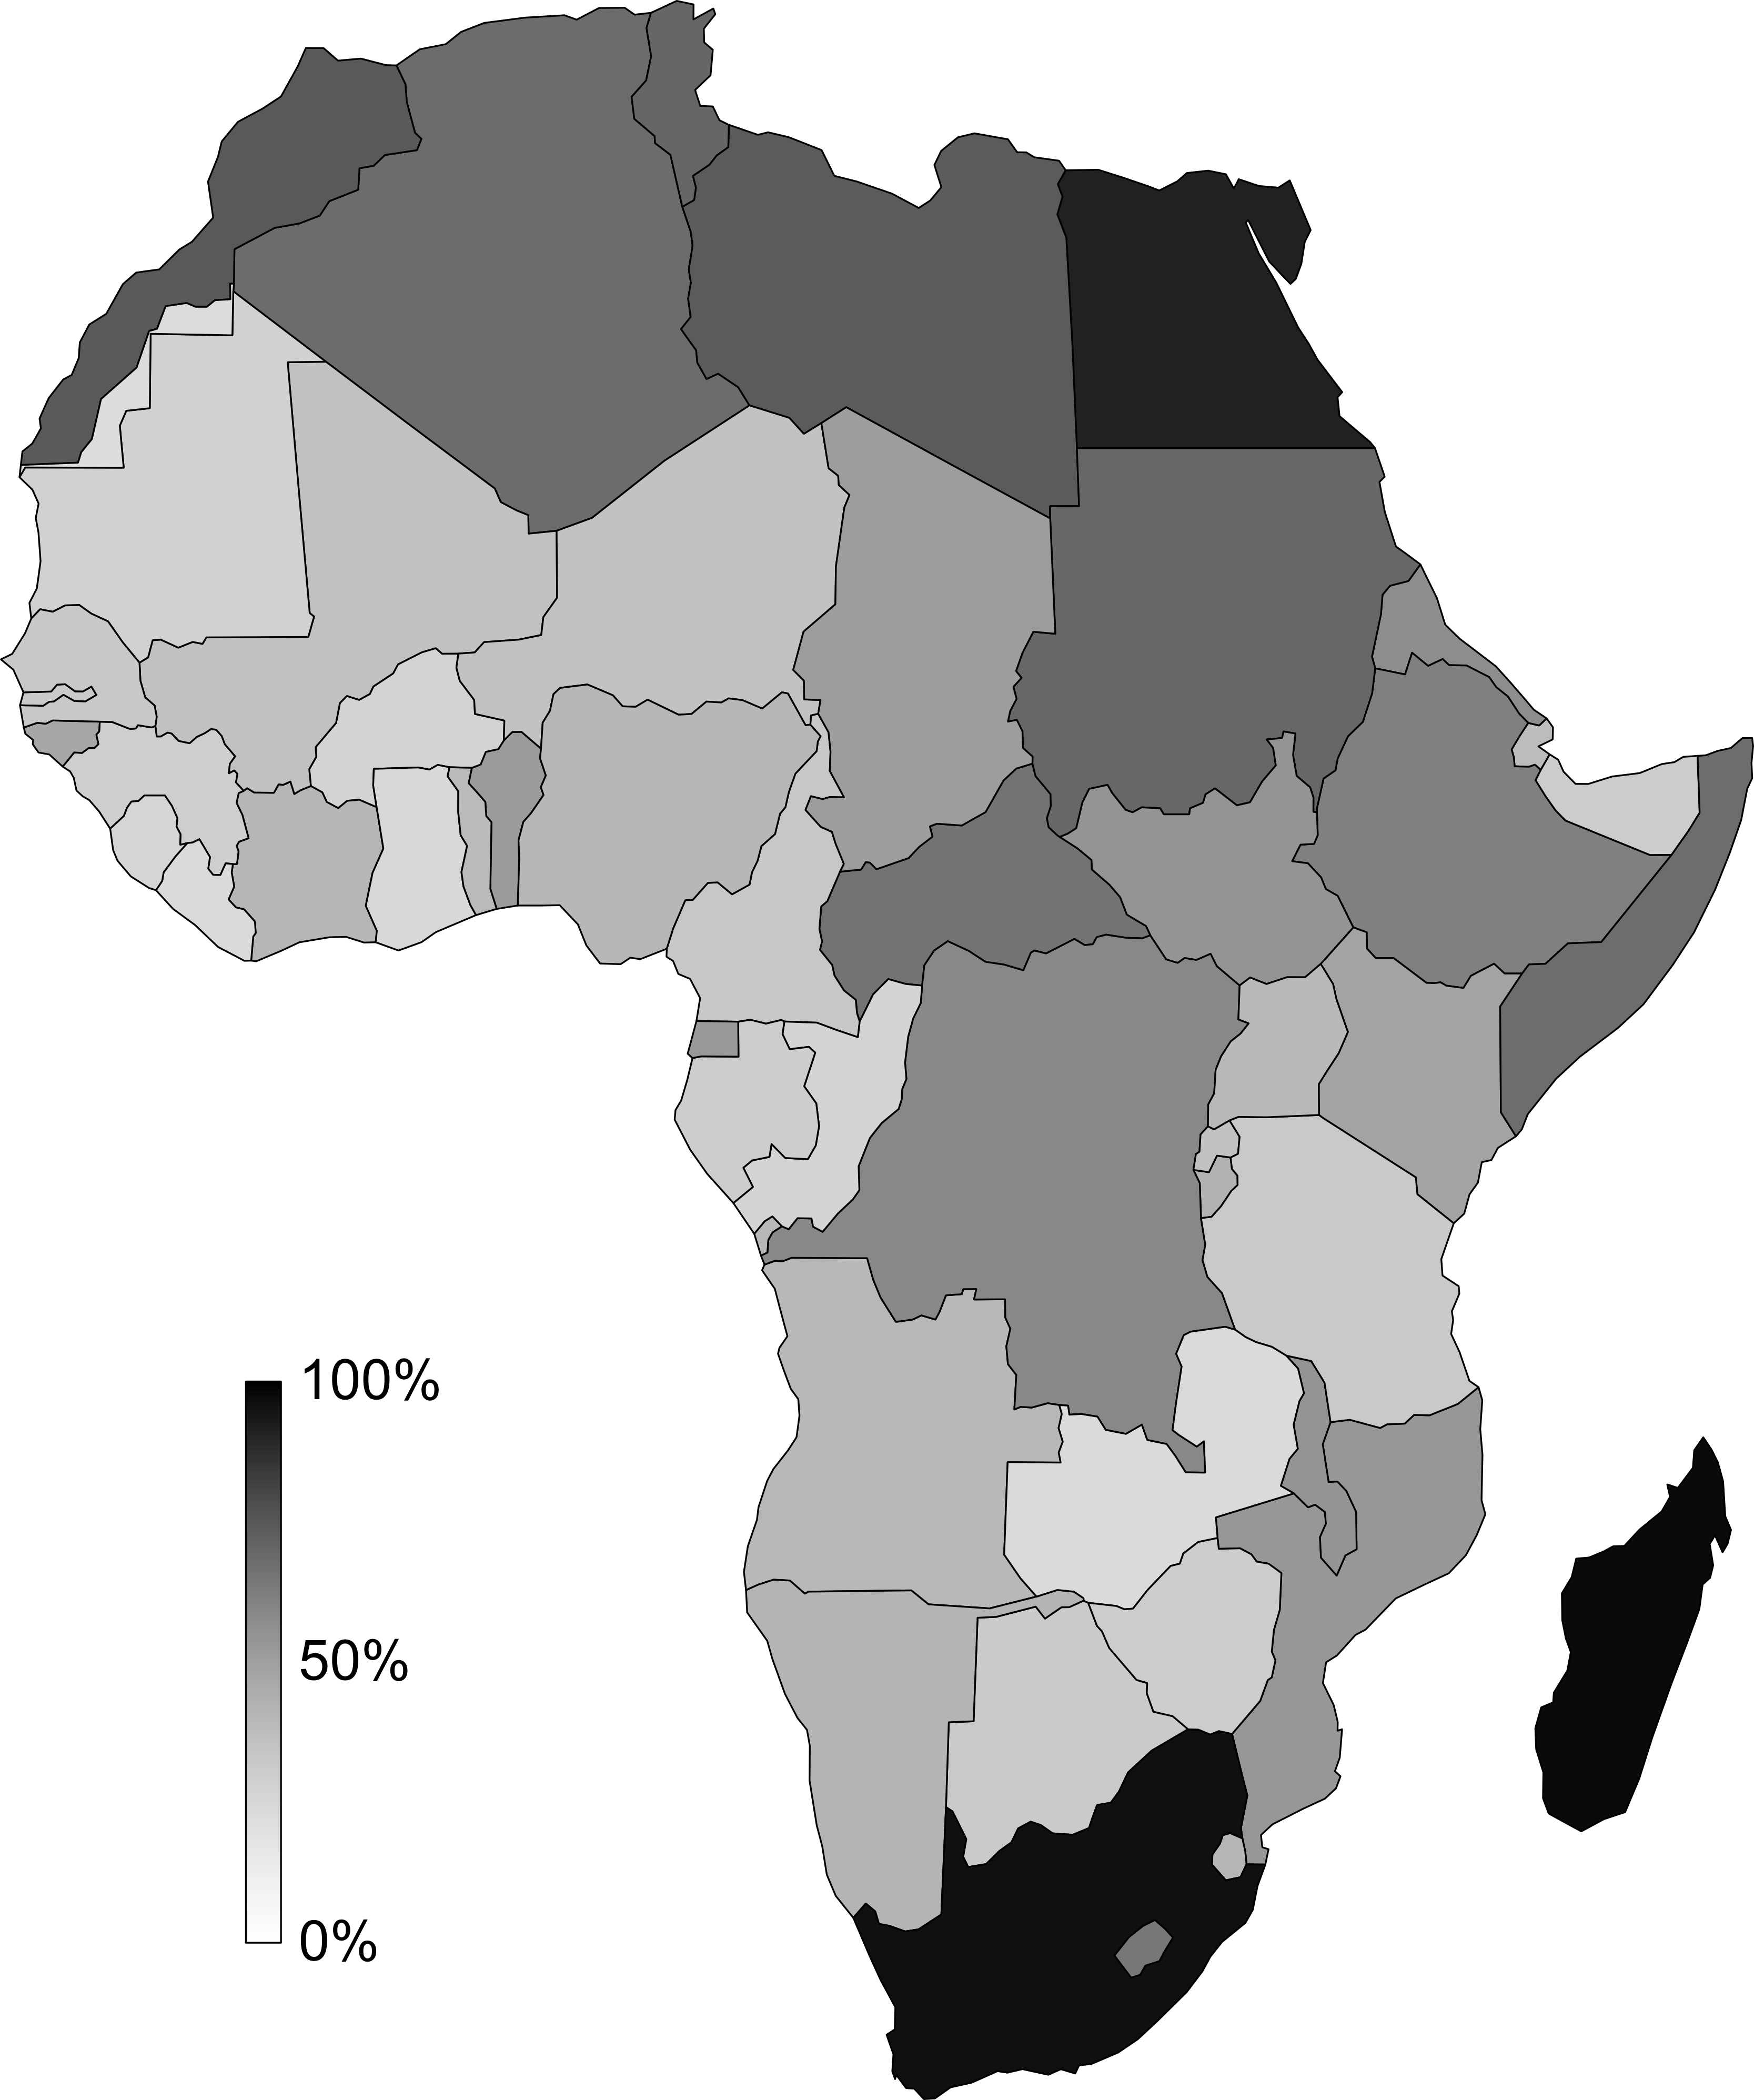
\includegraphics[width=.8\linewidth]{edm-2014-geography-models/africa-with-scale}

  \caption{Map of Africa colored by prior knowledge of countries, the shade
    corresponds to the probability of correct answer for an average user of
    \texttt{slepemapy.cz}. }
  \label{fig:africa}
\end{figure}

To achieve effective learning in domains such as geography it is necessary to
address several interrelated issues, particularly the estimation of knowledge,
the modeling of learning, the memory effects (spacing and forgetting), and the
question selection.

The above-mentioned issues have been studied before, but separatedly in different
context. Adaptation has been studied most thoroughly in the context of
\emph{computerized adaptive testing} (CAT) with the use of the item response
theory~\cite{de2008theory}. In CAT the goal is the testing, i.e. to determine
the skill of students. Therefore, the focus of CAT is on precision and statistical
guarantees. It usually does not address learning (students' skill is not
expected to change during a test) and motivation. In our setting the primary
goal is to improve the skill; estimation of the skill is only a secondary goal which
helps to achieve the main one. Thus the statistical accuracy of the estimation
is not so fundamental as it is in CAT. On the other hand, the issues of learning,
forgetting, and motivation are crucial for adaptive practice.

Another related area is the area of \emph{intelligent tutoring
systems}~\cite{vanlehn2006behavior}. These systems focus mainly on learning of
more complex cognitive skills than learning of facts, e.g. mathematics or
physics. The modeling of learning is widely studied in this context, particularly
using the popular Bayesian knowledge tracing model~\cite{corbett1994knowledge}.
A lot of research focuses on the acquisition of skills, less attention is given to
the prior knowledge and the forgetting (see e.g.~\cite{pardos2010modeling,qiu2011does}).

The learning of facts is well studied in the research of \emph{memory}, e.g. in the
study of spacing and forgetting effects~\cite{pavlik2005practice} and spaced
repetition~\cite{karpicke2007repeated}. These studies are not, however, usually
done in a realistic learning environment, but in a laboratory
and in areas with little prior knowledge, e.g. learning of arbitrary word
lists, nonsense syllables, obscure facts, or Japanese
vocabulary~\cite{delaney2010spacing,pavlik2005practice}. Such approach
facilitates interpretation of the experimental results, but the developed
models are not easily applicable in educational setting, where prior knowledge
can be an important factor. There are also many implementations of the spaced
repetition principle using ``flashcard software'' (well known example is
SuperMemo), but these implementations usually use scheduling algorithms with
fixed ad-hoc parameters and do not try to learn from collected data (or only
in a limited way). The spaced repetition was also studied specifically for
geography~\cite{zirkle2010effects}, but only in a simple setting.

In this work we propose both a general structure and a specific realization of
a computerized adaptive practice system for learning of facts. We have implemented
an instance of such system for learning geography, particularly names of
countries (\texttt{slepemapy.cz}, the system is so far implemented only in
Czech). Data from this system are used for the evaluation (over 2\,500
students, 250\,000 answers). To make the description more concrete and
readable, we sometimes use the terminology of this system, i.e., learning of
country names. Nevertheless, the approach is applicable to many similar domains
(other geographical objects, anatomy, biology, foreign vocabulary).

The functionality of the system is simple: it provides series of questions
about countries (``Where is country X?'', ``What is the name of this
country?'') and students answer them using an interactive map. Questions are
interleaved with a feedback on the success rate and a visualization of the
estimated knowledge of countries. The core of the system lies in estimating
students' knowledge and selecting suitable questions.

We decompose the design of such system into three steps and treat each of these
steps independently:
\begin{enumerate}
\item \emph{Estimation of prior knowledge}. Estimating the probability that a
  student $s$ knows a country $c$ before the first question about this country.
  The estimate is based on previous answers of the student $s$ and on answers
  of other students about the country $c$.
\item \emph{Estimation of current knowledge}. Estimating the probability that
  the student $s$ knows a country $c$ based on the estimation of prior
  knowledge and a sequence of previous answers of student $s$ on question about
  country $c$.
\item \emph{Selection of question}. Selection of a suitable question for a student
  based on the estimation of knowledge and the recent history of answers.
\end{enumerate}
Each of these issues is described and evaluated in a single section. The
independent treatment of these steps is a useful simplifications, since it
makes the development of the system and student models more tractable.
Nevertheless, it is clearly a simplification and we discuss limitations of this
approach in the final section.

%}}}

%{{{ background

\section{Background}

In this section we briefly describe some of the relevant models that are used
in the realization and evaluation of our approach.

\subsection{Bayesian Knowledge Tracing}

Bayesian knowledge tracing (BKT)~\cite{corbett1994knowledge,van2013properties}
is a well-known model for modeling of learning (changing skill). It is a hidden
Markov model where skill is the binary latent variable (either learned or
unlearned). The model has 4 parameters\footnote{BKT can also include
  forgetting. The described version corresponds to the variant of BKT that is
  most often used in research papers.}: probability that the skill is initially
learned, probability of learning a skill in one step, probability of incorrect
answer when the skill is learned (slip), and probability of correct answer when
the skill is unlearned (guess). The skill estimated is updated using a Bayes
rule based on the observed answers. Parameter estimation can be done using
the Expectation Maximization algorithm or using the exhaustive search.

\subsection{Rasch Model}

Basic model in the item response theory is the Rasch model (one parameter logistic
model). This model assumes the student's knowledge is constant and
expressed by a skill parameter $\theta$, the item's difficulty is expressed by a
parameter $b$, and the probability of a correct answer is given by the logistic
function:
\[ P(\mathit{correct}|b,\theta) = \frac{1}{1+e^{-(\theta-b})} \]
The standard way to estimate the parameters from data is to use the joint maximum
likelihood estimation~\cite{de2008theory}, which is an iterative procedure. In
the case of multiple choice question with $n$ options, the model is modified to
use a shifted logistic function:
\[ P(\mathit{correct}|b,\theta) = \frac{1}{n} +
(1-\frac{1}{n})\frac{1}{1+e^{-(\theta-b})} \]

\subsection{Performance Factor Analysis}

Performance factor analysis (PFA)~\cite{pavlik2009performance} can be seen as
an extension of Rasch model with changing skill. The skill, which is a logit of
probability of a correct answer, is given by a linear combination of the item's
difficulty and the past successes and failures of a student:
\[ P(\mathit{correct}) = \frac{1}{1+e^{-m}} \]
\[ m = \beta + \gamma s + \delta f \] where $\beta$ is the item difficulty, $s$
and $f$ are counts of previous successes and failures of the student, $\gamma$
and $\delta$ are parameters that determine the change of the skill associated with
correct and incorrect answer. Note that originally
PFA~\cite{pavlik2009performance} is formulated in terms of vectors, as it uses
multiple knowledge components; for our analysis the one-dimensional version is
sufficient.

\subsection{Elo System}

The Elo rating system~\cite{elo1978rating} was originally devised for chess
rating, i.e. estimating players skills based on results of matches. For each
player $i$ we have an estimate $\theta_i$ of his skill, based on the result $R$
(0 = loss, 1 = win) of a match with another player $j$; the skill estimate is
updated as follows:
\[ \theta_i := \theta_i + K(R-P(R=1))\] where $P(R=1)$ is the expected
probability of winning given by the logistic function with respect to the
difference in estimated skills, i.e. $P(R=1) = 1/(1+e^{-(\theta_i-\theta_j)})$,
and $K$ is a constant specifying sensitivity of the estimate to the last
attempt. An intuitive improvement, which is used in most Elo extensions, is to
use an ``uncertainty function'' instead of a constant $K$. There are several
extension to the Elo system in this direction, the most well-known is
Glicko~\cite{glickman1999parameter}.

We can use the Elo system in student modeling, if we interpret a student's answer
on an item as a ``match'' between the student and the item. Recently, several
researchers have studied this kind of application of the Elo system in
the educational data
mining~\cite{klinkenberg2011computer,wauters2010adaptive,wauters2011monitoring}.

The basic Elo system (reinterpreted in the context of educational
problems) also uses the logistic function and one parameter for each student and
problem. Thus the Rasch model and the Elo system are in fact very similar models,
the main principal difference is that the Rasch model assumes the constancy of
parameters, the Elo system assumes a changing skill.

%}}}

%{{{ est. prior knowledge

\section{Estimation of Prior Knowledge}

At first, we treat the estimation of prior knowledge. Our aim is to estimate
the probability that a student $s$ knows a country $c$ based on previous
answers of students $s$ to questions about different countries and previous
answers of other students to questions about country $c$ -- as a simplification
(for an easier interpretation of data) we use only the first answer about each
country for each student in this step.

%{{{ model

\subsection{Model}

In the following text we use a key assumption that both students and studied facts
are homogenous; we assume that we can model students' overall prior knowledge in
the domain by a one-dimensional parameter. This assumption is reasonable for
geography and students from Czech Republic (which is the case of our
application), but would not hold for geography and mixed population or for a mix
of facts from geography and chemistry. If the homogenity is not satisfied, we
can group the students and facts into homogenous groups (e.g. students by their
IP address, facts by an expert or by an automatic technique~\cite{aied13}) and
then make predictions for each subgroup independently.

More specifically, we model the prior knowledge by the Rasch model, i.e. we
have student parameter $\theta_s$ corresponding to the global knowledge of a
student $s$ of geography, the item parameter $b_c$ corresponding to the difficulty
of a country $c$, and the probability of a correct first answer is given by the
logistic function $P(\mathit{correct}|s,c) = \frac{1}{1+e^{-(\theta_s -
    b_c)}}$.

As we mentioned above, the standard approach to the parameter estimation for the
Rasch model is joint maximum likelihood estimation (JMLE). This is an iterative
approach that is slow for large data, particularly it is not suitable for
an online application, where we need to adjust estimates of
parameters continuously.

Therefore, we also consider the application of the Elo rating system in this
setting. Although the assumptions in this context are closer to the assumptions
of the Rasch model (the global skill and the difficulty of items are rather
constant), the Elo system is much more suitable for an online application and
results with simulated data suggest that it leads to similar
estimates~\cite{decayelo}.

%}}}

%{{{ evaluation

\subsection{Evaluation}

\begin{figure*}[t]
  \centering

  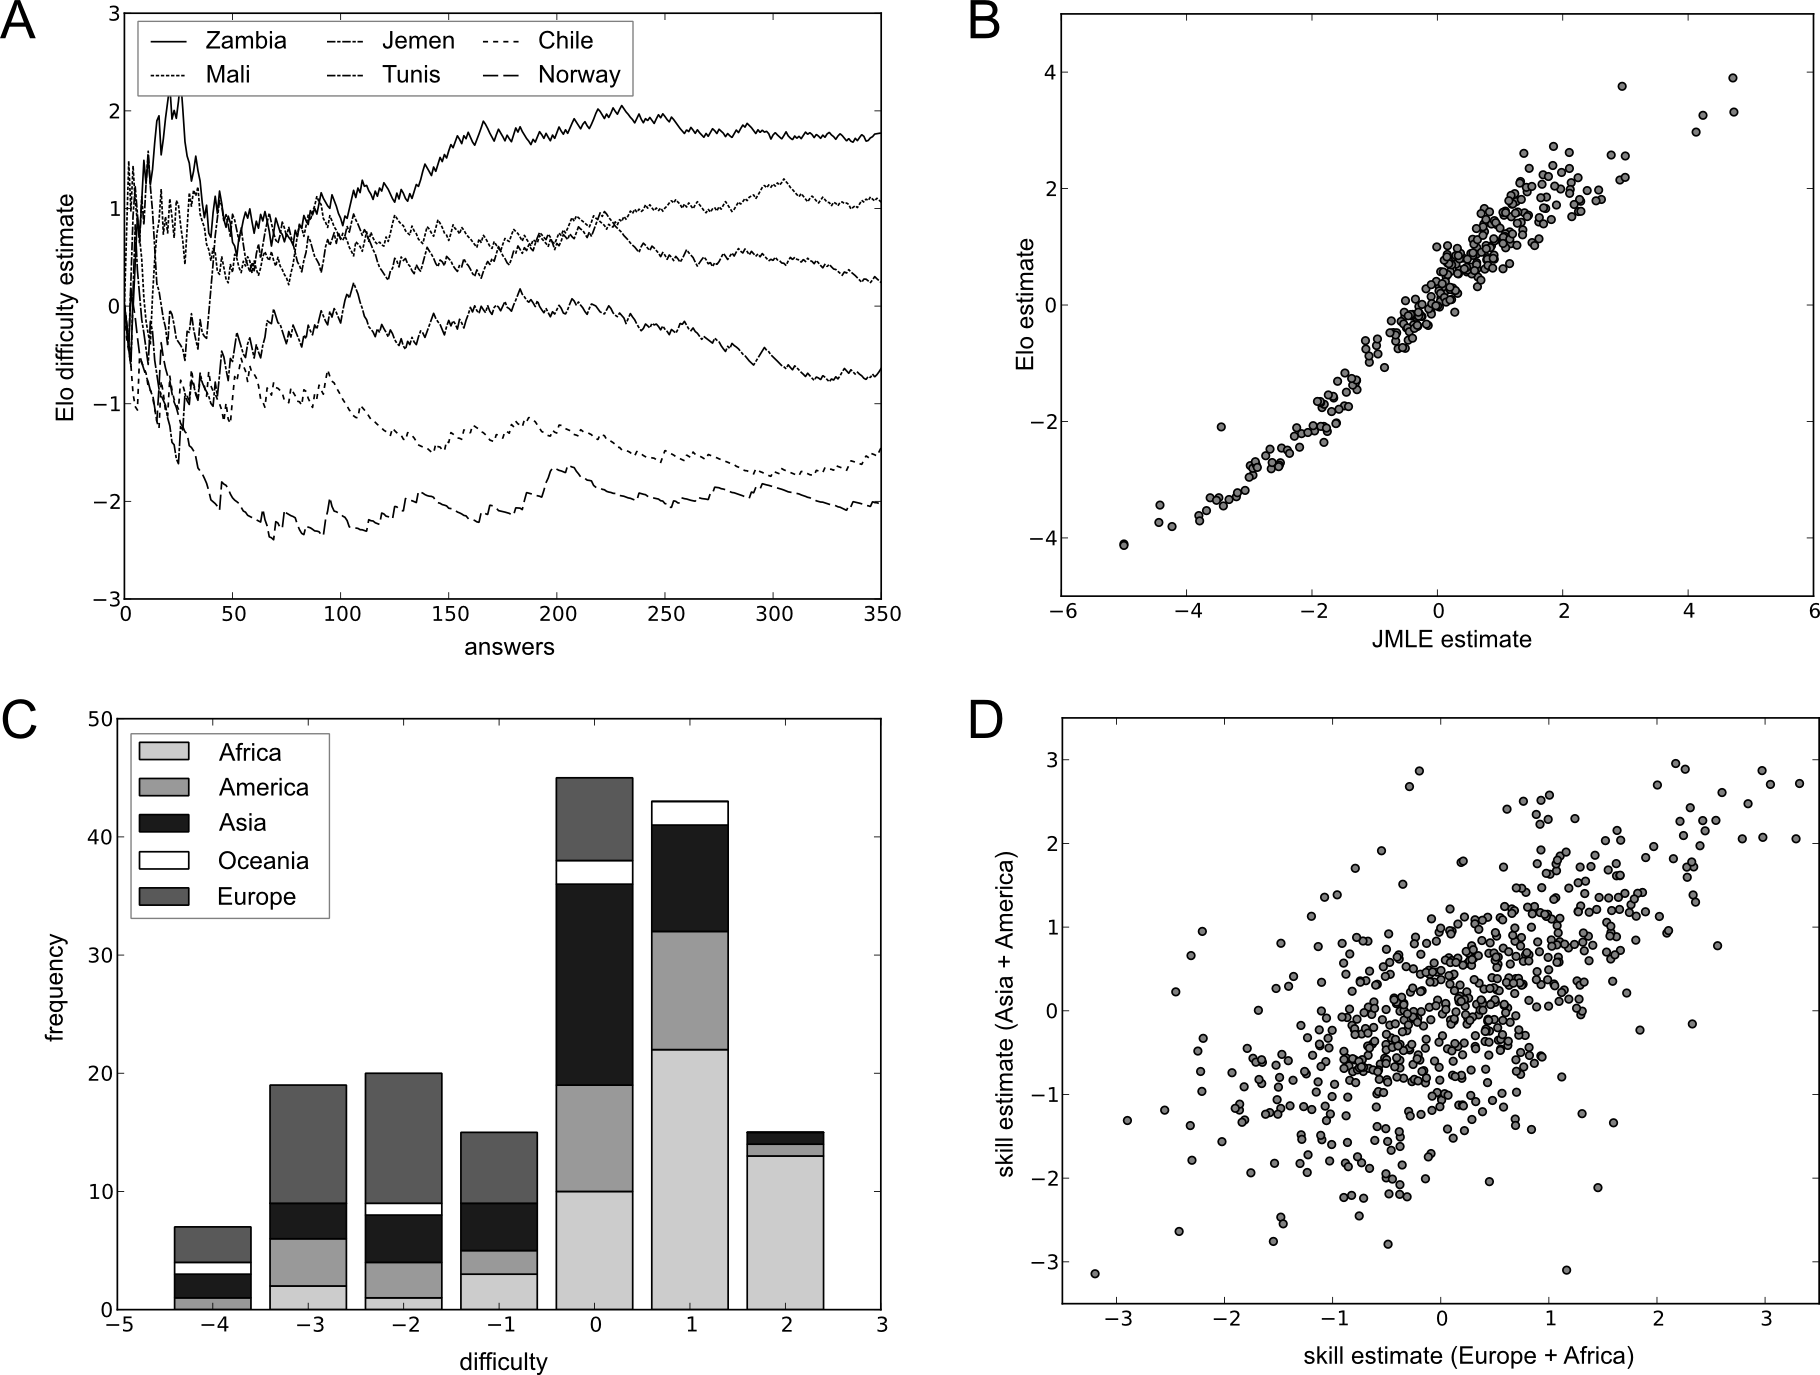
\includegraphics[width=\linewidth]{edm-2014-geography-models/prior-knowledge-fig}

  \caption{Estimation of prior knowledge: A) Development of estimates of
    difficulty of selected countries under Elo system, B) Comparison of Elo
    and JMLE difficulty estimates, C) Histogram of difficulty of countries, D)
    Correlation of ``subskills'' computed for different sets of countries.}
  \label{fig:prior-knowledge-eval}
\end{figure*}

The basic version of the Elo system with the constant update parameter $K$ does
not provide a good estimation -- if the parameter $K$ is small, the system takes
long to learn skills and difficulties, if the parameter $K$ is large, the
behavior of the system is unstable (estimates are too dependent on a last few
answers). Therefore, instead of the constant $K$ we use an uncertainty function
$\frac{a}{1+bn}$, where $n$ is the order of the answer and $a,b$ are
parameters. Using a grid search we have determined optimal values $a=1,
b=0.05$. This exact choice of parameter values is not important, many different
choices of $a,b$ provide very similar results.

This variant of the Elo system provides both fast coarse estimates after a few
answers and stability in the long run (see
Figure~\ref{fig:prior-knowledge-eval}~A). It also provides nearly identical
estimates as the joint maximum likelihood estimation
(Figure~\ref{fig:prior-knowledge-eval}~B, correlation 0.97). JMLE is
computationally demanding iterative procedure, the Elo system requires a single
pass of the data and can be easily used online. Since the estimates of the two
methods are nearly identical, we conclude that the Elo system is preferable in
our context.

Distribution of the difficulty parameters
(Figure~\ref{fig:prior-knowledge-eval}~C) reflects the target domain and
student population. In our case the difficulty of countries for Czech students
is skewed towards very easy items, which are mostly European countries.
Difficult countries are mostly African. Skill parameters are distributed
approximately normally.

We have tested the assumption of a single global skill by computing the skill for
independent subsets of items (countries from different continents) and then
checking the correlation between the obtained skill.
Figure~\ref{fig:prior-knowledge-eval}~D shows the results for two such
particular ``subskills'', the correlation coefficient for this case and other
similar pairs of subskills is around 0.6. Given that there is some intrinsic
noise in the data and that the skills are estimated from limited amount of
questions, this is quite high correlation. This suggests that the assumption of
a global skill is reasonable.

%}}}

%}}}

%{{{ est. of current knowledge

\section{Estimation of Current Knowledge}

We now turn to the estimation of a student's current knowledge, i.e. knowledge
influenced by the repeatedly answering of questions about a country. The input
data for this estimation are an estimate of prior knowledge (provided by the
above described model) and the history of previous attempts, i.e. the sequence
of previous answers (correctness of answers, question types, timing
information).

%{{{ models

\subsection{Models}

Several different models can be considered for the estimation of current
knowledge. Bayesian knowledge tracing can be used in a straightforward way. In
this context the probability of initial knowledge is given by the previous
step. The probability of learning, guess, and slip are either given by a context
(guess in the case of multiple choice question) or can be easily estimated
using an exhaustive search. However, in this context the assumptions of BKT are
not very plausible. BKT assumes a discrete transition from the unknown to the known
state, which may be reasonable a simplification for procedural skills, but for
declarative facts the development of the memory is gradual.

Assumptions of the Performance factor analysis are more relevant for the
learning of facts. Instead of the item difficulty parameter $\beta_i$, used in
the original version of PFA, we can use the estimate of the initial knowledge
for a student $s$ and a country $c$ in our setting. This is given by the
difference $\theta_s - b_c$.

A disadvantage of PFA is that it does not consider the order of answers (it
uses only the summary number of correct and incorrect answers) and it also does
not take into account the probability of guessing. Guessing can be important
particularly in our setting, where the system uses multiple choice questions
with variable number of options. To address these issues we propose to combine
PFA with some aspects of the Elo system (in the following text we denote this
version as PFAE -- PFA Elo/Extended):
\begin{itemize}
\item $K_{sc}$ is the estimated knowledge of a student $s$ of a country $c$.
\item The initial value of $K_{sc}$ is provided by the estimation of prior
  knowledge: $K_{sc} = \theta_s - b_c$.
\item The probability of correct answer to a question with $n$ options is given by
  the shifted logistic function:
\[ P(\mathit{correct}|K_{sc}, n) = \frac{1}{n} + (1-\frac{1}{n})\frac{1}{1+e^{-K_{sc}}} \]
\item After a question with $n$ options was answered, the estimated
  knowledge is updated as follows:
  \begin{itemize}
  \item $K_{sc} := K_{sc} + \gamma \cdot (1-P(\mathit{correct}|K_{sc}, n))$, if
    the answer was correct,
  \item $K_{sc} := K_{sc} + \delta \cdot P(\mathit{correct}|K_{sc}, n)$, if
    the answer was incorrect.
  \end{itemize}
\end{itemize}

The estimation can be further improved by taking into account the timing
information. If two questions about the same item are asked closely one after
another, then it can be expected that the student will answer the second one
correctly, because the answer is still in his short term memory. In models
based on a logistic function (PFA, PFAE) we can model this effect in the
following way: the skill is ``locally'' increased by $\frac{w}{t}$, where $t$
is the time (in seconds) between attempts and $k$ is a suitable constant
(optimal $w = 80$ for our data). It should be possible to further improve the
model by a more thorough treatment of forgetting and spacing effects, e.g., by
incorporating some aspects of the ACT-R model~\cite{pavlik2005practice}.

Another useful timing information is the response time. As the response time
tends to be log-normally distributed~\cite{its12,van2006lognormal}, we work
with the logarithm of time. Intuitively, the higher knowledge of a country
leads not only to higher probability of a correct answer, but also to a faster
response. Figure~\ref{fig:timing-information} shows results of an experiment
supporting this intuition -- distribution of times of correct answers is
shifted to lower values if the next answer on the same country is correct. This
suggests that response time could be used to improve the estimation of
knowledge. Indeed, even simple modification of the $\gamma$ parameter in the
PFA model (by comparison of the response time to mean response time) leads to a
slight improvement in predictions. A more involved application of the response
time requires a suitable normalization due to different speeds of students and
different sizes of countries -- it is much easier to click on China than on
Vietnam.

\begin{figure}[t]
  \centering

  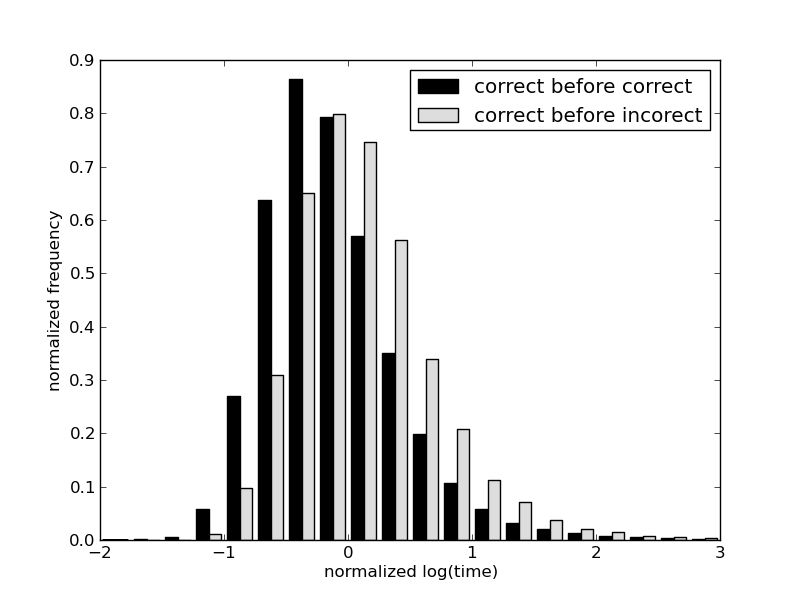
\includegraphics[width=\linewidth]{edm-2014-geography-models/response-time-pattern-gray}
  \caption{Normalized logarithm of time of correct answers, depending on
    whether the next answer about the country is answered correctly or
    incorrectly. }
  \label{fig:timing-information}
\end{figure}

%}}}

%{{{ evaluation

\subsection{Evaluation}

The described models provide predictions of probability of a correct answer. To
evaluate these models we need to choose a metric by which we measure
performance of models. In educational data mining researchers often provide
evaluation with respect to a chosen metric without providing any rationale for
the particular choice. In some cases the choice of metric is not fundamental
and different metrics lead to similar results (that is the case for above
described experiments with estimating prior knowledge). However, the evaluation
of models of the current knowledge is sensitive to the choice of a metric, and
thus it is necessary to pay attention to this issue.

Let us review the most commonly used metrics in educational data mining and
their suitability in our context. The mean absolute error (MAE) is not a good
metric, since for unbalanced data it prefers models skewed towards the larger
class. Consider a simulated student that answers correctly with constant
probability 0.7. If we optimize a constant predictor with respect to the mean
absolute error, the predicted probability is 1. The root mean square error
(RMSE) is a similar measure that does not share this disadvantage and is thus
preferable. The log-likelihood (LL) metric behaves similarly to RMSE except for
predictions very close to 0 or~1. Since LL is unbounded, a single wrong
prediction can degrade the performance of a model. To prevent this behaviour,
an ad-hoc bound can be introduced in the computation of LL. Metrics like AIC
and BIC are extensions of the log-likelihood penalizing large number of model
parameters. All models described above have only very small number of
parameters, and thus these metrics are not relevant for the current discussion.
Another popular metric is the area under the receiver operating characteristic
curve (AUC). This metric considers the prediction only in relative way -- note
that if all predictions are divided by 2, the AUC metric stays the same. In our
application, however, the precision of the absolute prediction is important,
since the value is used in computations that determine the choice of questions
and number of options in multiple choice questions.

Thus it seems that the most suitable metrics from the commonly used ones is
RMSE. Thus we use RMSE as our primary metric, i.e. to optimize values of model
parameters. Table~\ref{tab:model-comparison} provides a comparison of different
models also for other metrics. We can see that the results are inconclusive
regarding the comparison of BKT and PFA, but the newly proposed extension PFAE
beats both the standard PFA and BKT models with respect to all three reported
metrics. The results also show that the consideration of timing information
further improves the performance of models.

%{{{ table comparison

\begin{table}[t]
  \centering
  \caption{Model comparison. }
  \label{tab:model-comparison}

  \begin{tabular}{lrrr}
    \toprule
    model & RMSE & LL & AUC \\ \midrule
BKT & 0.262 & -42048 & 0.668 \\
PFA & 0.265 & -44740 & 0.669 \\
PFA + time & 0.262 & -43088 & 0.695 \\
PFAE & 0.262 & -41947 & 0.682 \\
PFAE + time & 0.259 & -40623 & 0.714 \\
    \bottomrule
  \end{tabular}
\end{table}

%}}}

% optimal parameter values

For the reported evaluation we use models with ``global'' parameters, i.e., for
example in the PFA and its extension we use the same parameters $\gamma,
\delta$ for all countries and students. Thus the models have very small number
of parameters (at most 4 for the extension with timing information) and can be
easily fit by an exhaustive search. Since the number of data points is many
orders larger (tens of thousands), overfitting is not an issue. It would be
possible to use the ``local'' parameter values for individual countries and
students, such variant would require an improved parameter estimation and a
mechanism for dealing with uneven distribution of data among countries and
students.

%}}}

%}}}

%{{{ question selection

\section{Question Selection}

We will now focus on the issue of the question selection. Based on the past
performance of the student we want to select a suitable next question. In the
context of our geography application the selection of a question consists of
several partial decisions: which country to target, which type of the
question to ask (``Where is X?'' versus ``What is the name of this
country?''), and how many options to give a student to choose from.

Compared to the knowledge estimation, the question selection is much harder to
evaluate, since we do not have a single, clear, easily measurable goal. The
overall goal of the question selection is quite clear -- it is the maximization
of student learning. But it is not easy to measure the fulfilment of this
general goal, since it depends also on the context of the learning. An
experiment with pre-test, post-test, and fixed time in the system may provide a
setting for an accurate evaluation of the different question selection
strategies. Results of such experiment would, however, lack ecological
validity, as many of the users of the system use the system on their own and
with variable time in the system, so for example the issue of motivation is
much more important than in a controlled experiment. A related
work~\cite{pavlik2008using} presents this kind of controlled experiment for
card selection in drill practice, the authors however provide comparison only
with respect to a very simple cyclic selection technique and not to an
evaluation of different alternatives of the selection algorithm. Another
possibility is to use the time spent in educational system as a measure of
quality of question selection. Here, however, the optimal choice with respect
to this measure may not be optimal for learning, see~\cite{lomas2013optimizing}
for a specific instance of an educational online game with this dynamics.

Thus at the moment we do not provide the evaluation of the question selection.
We formulate general criteria that the question selection should satisfy and
propose a specific approach to achieve these criteria.

\subsection{Criteria}

The question selection process should satisfy several criteria, which are
partly conflicting. The criteria and their weight may depend on the particular
application, the target student population, and student goals. We propose the
following main criteria.

The selection of question should depend on an estimated \emph{difficulty} of
question. From the testing perspective, it is optimal to use questions with
expected probability of a correct answer reaching 50\%, because such question
provide most information about students' knowledge. However, 50\% success rate
is rather low and for most students it would decrease motivation. Thus in our
setting (adaptive practice) it is better to aim for a higher success rate. At
the moment we aim at 75\%, similarly to previous
work~\cite{jansen2013influence}.

Another important issue is the \emph{repetition} of questions. This aspect
should be governed by the research about spacing effects
\cite{delaney2010spacing,pavlik2005practice}, particularly it is not sensible
to repeat the same question too early.
% take into account correctness of the
% answer -- if answered incorrectly, repeat soon, if correctly, repeat later
% (even if not cognitively fundamental, this is expected behaviour from the user
% point of view). .... not used at the moment TODO in FW

It may be also welcome to have \emph{variability} of question types. Different
question types are useful mainly as a tool for tuning the difficulty of
questions, but even if this is not necessary, the variability of question types
may be meaningful criteria in itself, since it improves user experience, if
used correctly.

\subsection{Selecting Target Country}

\begin{figure*}
	\centering

        
\includegraphics[width=\linewidth]{edm-2014-geography-models/score-functions}

	\caption{Desired contribution of different criteria to selection of
          target country.}
	\label{fig:score-functions}
\end{figure*}

We propose to use the linear scoring approach to select a target country (the
correct answer of the question). For each relevant attribute, we consider a
scoring function that expresses the desirability of a given country with respect
to this attribute. These scoring functions are combined using weighted sum, the
country with highest total score is selected as a target. We consider the
following attributes:
\begin{enumerate}
\item the probability the student knows the country,
\item time since the last question about the country,
\item the number of questions already answered by the student about the country.
\end{enumerate}

Figure~\ref{fig:score-functions} shows the general shape of scoring functions
for these attributes. Further we specify concrete formulas that
approximate these shapes using simple mathematical functions.

The first case takes into account the relation between the estimated
probability of a correct answer ($P_{\mathit{est}}$) and the target success
rate ($P_{\mathit{target}}$). Assume that our goal is to ask a question where
the student has 75\% chance of a correct answer. The distance from the
probability for the difficult countries (nearly 0\% chance of the correct
answer) is higher than for easy ones (almost 100\%), so it is necessary to
normalize it.
\begin{displaymath}
  S_\mathit{prob}(P_\mathit{est}, P_\mathit{target}) =
  \left\{  \begin{array}{ll}
      \frac{P_{\mathit{est}}}{P_{\mathit{target}}}  & \mbox{if } P_{\mathit{target}} \geq P_{\mathit{est}} \\
      \frac{1 - P_{\mathit{est}}}{1 - P_{\mathit{target}}} & \mbox{if } P_{\mathit{target}} < P_{\mathit{est}}
    \end{array}
  \right.
\end{displaymath}
The second scoring function penalizes countries according to the time elapsed
since the last question, because we do not want to repeat countries in a short
time interval when they are still in short term memory. We use the function
$S_{time}(t) = - 1/t$, where $t$ is time in seconds. Using just the above
mentioned attributes the system would ask questions for only a limited pool of
countries. To induce the system to ask questions about new countries we
introduce the third scoring function that uses the total number $n$ of
questions for the given country answered by the student: $S_\mathit{count}(n) =
1/\sqrt{1 + n}$. The total score is given as a weighted sum of individual
scores, the weights are currently set manually, reflecting experiences with the
system: $W_\mathit{prob} = 10$, $W_\mathit{count} = 10$, $W_\mathit{time} =
120$.

% $S = W_\mathit{prob}\cdot
%S_\mathit{prob} + W_\mathit{count}\cdot S_\mathit{count} + W_\mathit{time}\cdot
%S_\mathit{time}$

\subsection{Choosing Options}

Once the question's target is selected, the question can be adjusted according
to the student's needs by using a multiple choice question with suitable number
of options. For a multiple choice question the probability of a correct answer
is the combination of the probability of guessing the answer
($P_\mathit{guess}$) and knowing the target country
($P_\mathit{est}$)\footnote{This is, of course, simplification since a multiple
  choice question can also be answered by ruling out distractor options. But if
  the distractors are well chosen; this simplification is reasonable. }:
\begin{displaymath}
  P_\mathit{success} = P_\mathit{guess} + (1 - P_\mathit{guess}) \cdot P_\mathit{est}
\end{displaymath}
As our goal is to get $P_\mathit{success}$ close to $P_\mathit{target}$, we
would like to make $P_\mathit{guess}$ close to
\begin{displaymath}
   G = \frac{P_\mathit{target} - P_\mathit{est}}{1 - P_\mathit{est}}
\end{displaymath}
For $G \leq 0$, we use open question (no options), otherwise we use $n$ closest
to $\frac{1}{G}$ as a number of options. For principal reasons the minimal
possible value of $n$ is 2, for practical reasons there is also an upper bound
for $n$ (more than 6 options would be confusing). The type of the question --
``Where is country X?'' or ``What is the name of this country?'' is currently
selected randomly. In case of an open question the first type is always used.

When using multiple choice questions, we also need to choose the distractor
options. Unlike other systems for practice dealing with
text~\cite{mitkov2006computer,mostow2002automated}, we work with well
structured data, so the problem of option selection is easier. The choice of
options can be based on domain information, e.g. geographically close
countries or countries with similar names. The easiest way to choose good
distractors is, however, to simply base the choice on past answers. We can take
countries most commonly mistaken with the target country (in open questions)
and select from them randomly. The random choice is weighted by the frequency
of mistakes with the given country, for example Kamerun is most often confused
with Niger (38\%), Nigeria (27\%), Central African Republic (10\%), Republic of
the Congo (9\%), Gabon (6\%), Ivory Coast (5\%), Uganda (3\%), and Guinea
(2\%).

%}}}

%{{{ discussion

%\newpage
\section{Discussion}

We described the functionality of the system in three independent parts: the
estimation of prior knowledge, the estimation of current knowledge, and the
selection of a question. The independent treatment of these steps is, however,
a simplification, as there is an interaction between these steps.

In our treatment, only the first answer about a given item is taken as an
indication of a prior knowledge, other answers are considered as an indication
of changes in knowledge. But for example the second answer, clearly, also
contains some information about prior knowledge. A more precise models should
be possible by incorporating more integrated approach to the estimation of
prior and current knowledge.

The selection of a question was treated as a subsequent step after the
estimation of knowledge, but in reality there is a feedback loop: the
estimation of knowledge influences the selection of a question and the
selection of a question determines the data that are collected and used for the
estimation of knowledge. Since the collected data are partially determined by
the model used, there may be a bias in the data towards certain questions, and
this bias may, in a subtle way, influence the evaluation. For example, if the
model overestimates the knowledge of students, the question selection stops
asking questions about items too early, which means that the system does not
collect data that would contradict the overestimated knowledge. The question
selection procedure may be also modified in such a way to collect data most
useful for improving the precision of the estimation. The study of these
interactions may be more important than differences between different models or
estimation procedures, which typically get most attention in current research
in student modeling.

% Another issue that deserves more attention than usually gets, is the choice of
% metric with respect to which model parameters are optimized and models
% compared. As our experience suggest, the choice of metric is not
% straightforward and it is an important issue, since different metrics may lead
% to different choice of models and parameter values, which then influence the
% behavior of the educational system.

%}}}

\subsection*{Acknowledgements}

Authors thank anonymous reviewers for valuable comments, Ji\v{r}\'i
\v{R}\'{i}h\'ak and Juraj Ni\v{z}nan for fruitful discussions, and Tereza
Dole\v{z}alov\'{a} for language assistance.

\bibliography{bibliography}

\end{document}
